\documentclass[tikz, border=10pt]{standalone}
\usepackage{pgfplots}
\usepackage{amsmath}
\usetikzlibrary{backgrounds}
\pgfplotsset{compat=1.18}

\begin{document}
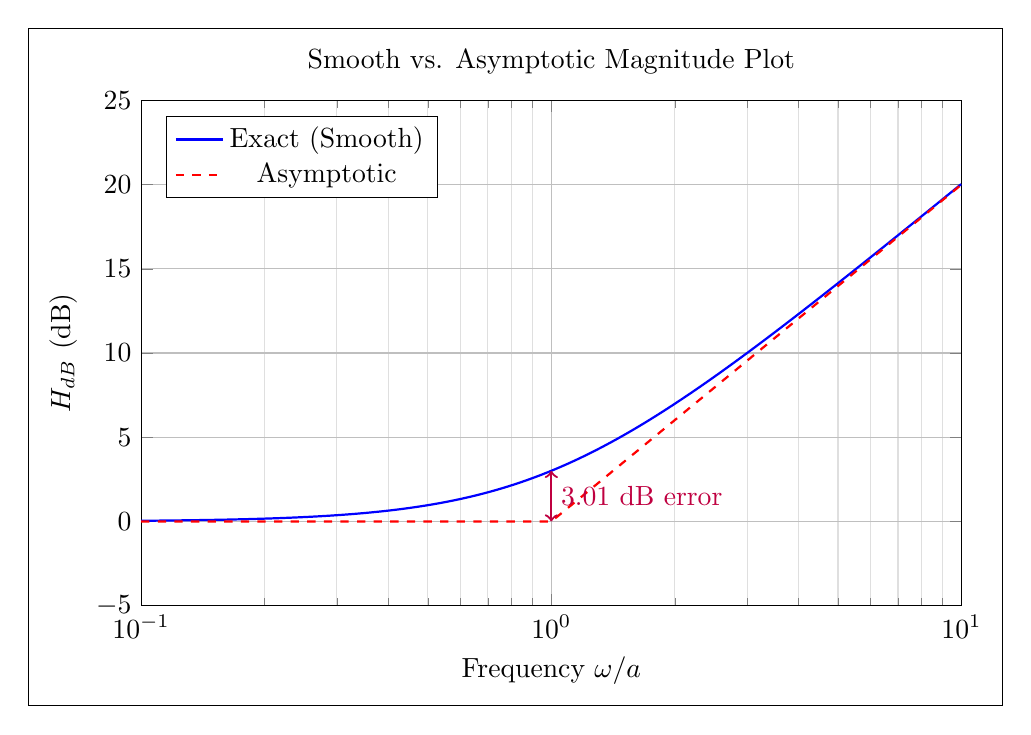
\begin{tikzpicture}[show background rectangle]
    \begin{semilogxaxis}[
        width=12cm, height=8cm,
        title={Smooth vs. Asymptotic Magnitude Plot},
        xlabel={Frequency $\omega/a$},
        ylabel={$H_{dB}$ (dB)},
        grid=both,
        xmin=0.1, xmax=10,
        ymin=-5, ymax=25,
        minor grid style={gray!25},
        major grid style={gray!50},
        legend pos=north west,
    ]

    % Exact: 20log10( sqrt(1 + (w/a)^2) )
    \addplot[blue, thick, domain=0.1:10, samples=200] { 10*log10( 1 + x^2 ) };
    \addlegendentry{Exact (Smooth)}

    % Asymptotic
    \addplot[red, dashed, thick] coordinates {
        (0.1, 0) (1, 0) (10, 20)
    };
    \addlegendentry{Asymptotic}

    % Annotate the error at w=a
    \draw[<->, purple, thick] (axis cs:1, 0) -- (axis cs:1, 3.01);
    \node[anchor=west, purple] at (axis cs:1, 1.5) {3.01 dB error};
    
    \end{semilogxaxis}
\end{tikzpicture}
\end{document}
